%%
%% This is file `sample-sigconf.tex',
%% generated with the docstrip utility.
%%
%% The original source files were:
%%
%% samples.dtx  (with options: `all,proceedings,bibtex,sigconf')
%%
%% IMPORTANT NOTICE:
%%
%% For the copyright see the source file.
%%
%% Any modified versions of this file must be renamed
%% with new filenames distinct from sample-sigconf.tex.
%%
%% For distribution of the original source see the terms
%% for copying and modification in the file samples.dtx.
%%
%% This generated file may be distributed as long as the
%% original source files, as listed above, are part of the
%% same distribution. (The sources need not necessarily be
%% in the same archive or directory.)
%%
%%
%% Commands for TeXCount
%TC:macro \cite [option:text,text]
%TC:macro \citep [option:text,text]
%TC:macro \citet [option:text,text]
%TC:envir table 0 1
%TC:envir table* 0 1
%TC:envir tabular [ignore] word
%TC:envir displaymath 0 word
%TC:envir math 0 word
%TC:envir comment 0 0
%%
%% The first command in your LaTeX source must be the \documentclass
%% command.
%%
%% For submission and review of your manuscript please change the
%% command to \documentclass[manuscript, screen, review]{acmart}.
%%
%% When submitting camera ready or to TAPS, please change the command
%% to \documentclass[sigconf]{acmart} or whichever template is required
%% for your publication.
%%
%%
\documentclass[sigconf,anonymous,review]{acmart}
\usepackage{listings}
\lstset{
  language=Python,
  basicstyle=\ttfamily\small,
  keywordstyle=\bfseries,
  commentstyle=\itshape,
  breaklines=true,
  frame=single,
  numbers=left,
  numberstyle=\tiny,
  xleftmargin=1.5em,
  framexleftmargin=1.5em
}
%%
%% \BibTeX command to typeset BibTeX logo in the docs
\AtBeginDocument{%
  \providecommand\BibTeX{{%
    Bib\TeX}}}

%% Rights management information.  This information is sent to you
%% when you complete the rights form.  These commands have SAMPLE
%% values in them; it is your responsibility as an author to replace
%% the commands and values with those provided to you when you
%% complete the rights form.
\setcopyright{acmlicensed}
\copyrightyear{2018}
\acmYear{2018}
\acmDOI{XXXXXXX.XXXXXXX}
%% These commands are for a PROCEEDINGS abstract or paper.
\acmConference[Conference acronym 'XX]{Make sure to enter the correct
  conference title from your rights confirmation email}{June 03--05,
  2018}{Woodstock, NY}
%%
%%  Uncomment \acmBooktitle if the title of the proceedings is different
%%  from ``Proceedings of ...''!
%%
%%\acmBooktitle{Woodstock '18: ACM Symposium on Neural Gaze Detection,
%%  June 03--05, 2018, Woodstock, NY}
\acmISBN{978-1-4503-XXXX-X/2018/06}


%%
%% Submission ID.
%% Use this when submitting an article to a sponsored event. You'll
%% receive a unique submission ID from the organizers
%% of the event, and this ID should be used as the parameter to this command.
%%\acmSubmissionID{123-A56-BU3}

%%
%% For managing citations, it is recommended to use bibliography
%% files in BibTeX format.
%%
%% You can then either use BibTeX with the ACM-Reference-Format style,
%% or BibLaTeX with the acmnumeric or acmauthoryear sytles, that include
%% support for advanced citation of software artefact from the
%% biblatex-software package, also separately available on CTAN.
%%
%% Look at the sample-*-biblatex.tex files for templates showcasing
%% the biblatex styles.
%%

%%
%% The majority of ACM publications use numbered citations and
%% references.  The command \citestyle{authoryear} switches to the
%% "author year" style.
%%
%% If you are preparing content for an event
%% sponsored by ACM SIGGRAPH, you must use the "author year" style of
%% citations and references.
%% Uncommenting
%% the next command will enable that style.
%%\citestyle{acmauthoryear}


%%
%% end of the preamble, start of the body of the document source.
\begin{document}

%%
%% The "title" command has an optional parameter,
%% allowing the author to define a "short title" to be used in page headers.
\title{SecMutBench: Evaluating LLM-Generated Security Tests via Mutation-Based Vulnerability Detection}

%%
%% The "author" command and its associated commands are used to define
%% the authors and their affiliations.
%% Of note is the shared affiliation of the first two authors, and the
%% "authornote" and "authornotemark" commands
%% used to denote shared contribution to the research.
\author{Ben Trovato}
\authornote{Both authors contributed equally to this research.}
\email{trovato@corporation.com}
\orcid{1234-5678-9012}
\author{G.K.M. Tobin}
\authornotemark[1]
\email{webmaster@marysville-ohio.com}
\affiliation{%
  \institution{Institute for Clarity in Documentation}
  \city{Dublin}
  \state{Ohio}
  \country{USA}
}

\author{Lars Th{\o}rv{\"a}ld}
\affiliation{%
  \institution{The Th{\o}rv{\"a}ld Group}
  \city{Hekla}
  \country{Iceland}}
\email{larst@affiliation.org}

\author{Valerie B\'eranger}
\affiliation{%
  \institution{Inria Paris-Rocquencourt}
  \city{Rocquencourt}
  \country{France}
}

\author{Aparna Patel}
\affiliation{%
 \institution{Rajiv Gandhi University}
 \city{Doimukh}
 \state{Arunachal Pradesh}
 \country{India}}

\author{Huifen Chan}
\affiliation{%
  \institution{Tsinghua University}
  \city{Haidian Qu}
  \state{Beijing Shi}
  \country{China}}

\author{Charles Palmer}
\affiliation{%
  \institution{Palmer Research Laboratories}
  \city{San Antonio}
  \state{Texas}
  \country{USA}}
\email{cpalmer@prl.com}

\author{John Smith}
\affiliation{%
  \institution{The Th{\o}rv{\"a}ld Group}
  \city{Hekla}
  \country{Iceland}}
\email{jsmith@affiliation.org}

\author{Julius P. Kumquat}
\affiliation{%
  \institution{The Kumquat Consortium}
  \city{New York}
  \country{USA}}
\email{jpkumquat@consortium.net}

%%
%% By default, the full list of authors will be used in the page
%% headers. Often, this list is too long, and will overlap
%% other information printed in the page headers. This command allows
%% the author to define a more concise list
%% of authors' names for this purpose.
\renewcommand{\shortauthors}{Trovato et al.}

\newcommand{\todo}[1]{\textcolor{red}{\textit{[TODO: #1]}}}

%%
%% The abstract is a short summary of the work to be presented in the
%% article.
\begin{abstract}
Evaluating whether Large Language Models (LLMs) can generate effective security tests remains an open challenge. Existing code security benchmarks focus on secure code \emph{generation} and rely on surface-level metrics such as pass@k, failing to measure whether generated tests actually detect vulnerabilities. We introduce SecMutBench, a mutation-based benchmark for evaluating LLM-generated security tests across 30 CWE categories. SecMutBench applies 25 security-specific mutation operators to 339 Python programs, producing 1,869 mutants that model realistic vulnerability patterns---such as converting parameterized SQL queries to string concatenation (CWE-89) or downgrading cryptographic algorithms (CWE-327). We propose the Security Mutation Score (SMS), which classifies mutant kills into semantic, functional, incidental, and crash categories using operator-aware heuristics to distinguish genuine security awareness from superficial test failures. Our evaluation of eight LLMs alongside static analysis baselines (Bandit, Semgrep) reveals a critical finding: accounting for test validity, the best LLM achieves only 19.7\% effective SMS (SMS $\times$ Secure-Pass Rate) compared to 47.6\% for expert-written reference tests---a 2.4$\times$ gap that raw mutation scores completely obscure. Among valid test suites, traditional mutation scores further overstate security capability by an average of 2.2$\times$ compared to SMS, with functional assertions and runtime crashes---not security-aware assertions---accounting for the majority of mutant kills. Furthermore, static analysis achieves 71.4\% detection on pattern-based vulnerabilities but 0\% on logic-flaw CWEs, demonstrating complementary coverage. SecMutBench is publicly available with an executable evaluation framework, CWE-specific mock environments, and pre-generated mutants for reproducible benchmarking.
\end{abstract}

%%
%% The code below is generated by the tool at http://dl.acm.org/ccs.cfm.
%% Please copy and paste the code instead of the example below.
%%
\begin{CCSXML}
<ccs2012>
<concept>
<concept_id>10011007</concept_id>
<concept_desc>Software and its engineering</concept_desc>
<concept_significance>500</concept_significance>
</concept>
</ccs2012>
\end{CCSXML}

\ccsdesc[500]{Software and its engineering}
%%
%% Keywords. The author(s) should pick words that accurately describe
%% the work being presented. Separate the keywords with commas.
\keywords{security benchmark, mutation testing, large language models, vulnerability detection, code security, CWE, LLM evaluation, software testing, security testing}
%% A "teaser" image appears between the author and affiliation
%% information and the body of the document, and typically spans the
%% page.


\received{20 February 2007}
\received[revised]{12 March 2009}
\received[accepted]{5 June 2009}

%%
%% This command processes the author and affiliation and title
%% information and builds the first part of the formatted document.
\maketitle

%% ====================================================================
%% I. INTRODUCTION
%% ====================================================================
\section{Introduction}

Software vulnerabilities remain one of the most costly challenges in modern computing. The global cost of cybercrime reached \$9.22 trillion in 2024 and is projected to exceed \$10.5 trillion in 2025~\cite{cybersecventures2025}, with the average cost of a single data breach climbing to \$4.88 million globally and \$10.22 million in the United States alone~\cite{ibm2024breach}. Unpatched vulnerabilities account for approximately 20\% of all breaches, while over 29,000 critical vulnerabilities were disclosed in 2025---a 24\% increase over the prior year. Security testing is fundamental to identifying these vulnerabilities before deployment, yet manual security test creation is expensive, time-consuming, and difficult to scale.

At the same time, AI-powered coding assistants have seen explosive adoption. According to Stack Overflow's 2025 Developer Survey~\cite{stackoverflow2025survey}, 84\% of developers now use AI tools in their workflows, with 65\% using them at least weekly and 51\% of professional developers relying on them daily. Code generation has become AI's first breakout use case, growing into a \$1.9 billion ecosystem~\cite{menlo2025llm} that includes AI IDEs (Cursor~\footnote{\url{https://cursor.sh}}, Windsurf~\footnote{\url{https://codeium.com/windsurf}}), application builders (Lovable, Bolt), and enterprise coding agents (Claude Code, GitHub Copilot~\cite{pearce2022asleep}). Major technology companies report that 25\% or more of their code is now AI-generated, and Menlo Ventures estimates that code-generation-focused AI captured 42\% of the LLM developer market by mid-2025~\cite{menlo2025llm}.

This rapid adoption introduces a critical question for software security: \emph{as LLMs increasingly generate code, can they also generate effective security tests to catch vulnerabilities in that code?} The stakes are high---if AI-generated code is deployed with inadequate security testing, the same tools that accelerate development may simultaneously accelerate vulnerability introduction.

Several benchmarks have emerged to evaluate LLM security capabilities, but they focus almost exclusively on secure code \emph{generation}. CyberSecEval~\cite{bhatt2023cyberseceval} evaluates whether LLMs produce vulnerable code completions across multiple languages, using static analysis rules for automated detection. SecurityEval~\cite{siddiq2022securityeval} provides 130 prompt-based Python coding challenges mapped to 75 CWE types, while SecCodePLT~\cite{secccodeplt2024} extends this with ground-truth secure/insecure code pairs and automated evaluation pipelines. CWEval~\cite{yang2024cweval} offers 119 expert-verified tasks across 31 CWE types with CodeQL-based detection, enabling outcome-driven evaluation of both functionality and security. More recently, CFCEval~\cite{cheng2025cfceval} introduced the Element-Level Relevance Metric (ELRM) to assess code fix quality across four dimensions, addressing dataset bias through the MLVBench benchmark. Pearce et al.~\cite{pearce2022asleep} assessed the security of GitHub Copilot's code contributions, finding that approximately 40\% of generated programs contained vulnerabilities. Tony et al.~\cite{tony2023llmseceval} created natural language prompts for security evaluations across multiple CWE categories.

A critical distinction separates all these benchmarks from SecMutBench: they focus on code \emph{generation} quality---evaluating whether LLM-produced code is secure. SecMutBench instead evaluates test \emph{generation} quality---measuring whether LLM-produced tests can detect vulnerabilities. These are complementary but fundamentally different capabilities. A model that generates secure code may still be unable to articulate \emph{what makes alternative implementations vulnerable} through targeted test assertions. Furthermore, a model may avoid generating vulnerable code simply because it has learned to produce safe patterns, without possessing any deeper understanding of the vulnerability mechanism.

This gap in evaluation is compounded by a gap in \emph{metrics}. Current approaches rely on surface-level measures---pass rates, code similarity scores (e.g., CodeBLEU), and binary pass/fail against known vulnerabilities---that cannot distinguish between a test that detects a SQL injection through a targeted assertion (\texttt{assert ``parameterized'' in query\_method}) and one that merely crashes when encountering malformed input (\texttt{TypeError: unsupported operand}). This distinction is critical in practice: a crash-inducing test provides no diagnostic value to a developer, while a security-aware assertion identifies the specific vulnerability class and suggests a remediation path. Yet no existing benchmark makes this distinction.

We address these gaps with SecMutBench, a mutation-based benchmark grounded in two decades of security mutation testing research~\cite{du2000testing,shahriar2008music,mouelhi2007mutation}. Rather than evaluating whether LLM-generated code is secure, we evaluate whether LLM-generated \emph{tests} can detect security vulnerabilities. Our approach applies 25 security-specific mutation operators that transform secure code into realistic vulnerable variants---such as converting parameterized SQL queries to string concatenation (CWE-89), replacing \texttt{subprocess.run([...])} with \texttt{shell=True} string commands (CWE-78), or downgrading SHA-256 to MD5 (CWE-327). Each mutant models a known vulnerability pattern mapped to a CWE category~\cite{mitre2024cwe}. LLM-generated tests are then evaluated against these mutants, and kills are classified by type---semantic, functional, incidental, or crash---to reveal whether models demonstrate genuine security awareness or merely detect code breakage.

Our evaluation reveals two striking findings. First, only 7--47\% of LLM-generated test suites even pass on secure code; accounting for this, the best model achieves only 19.7\% effective security mutation score compared to 47.6\% for expert-written tests---a 2.4$\times$ gap that raw metrics completely obscure. Second, among valid test suites, traditional mutation scores further overstate capability by an average of 2.2$\times$, with functional assertions and runtime crashes---not security-aware assertions---accounting for the inflation. These compounding distortions mean that a model reporting 90\% mutation score may deliver only 5\% effective security detection in practice.

Our key contributions are:

\begin{enumerate}
    \item \textbf{SecMutBench benchmark}: 339 Python programs across 30 CWE categories with 25 mutation operators producing 1,869 pre-generated mutants from curated data sources (SecCodePLT, CyberSecEval, SecurityEval, CWEval, hand-crafted templates, and LLM-generated variations), accompanied by an executable evaluation framework with 11 CWE-specific mock environments, a \texttt{SafeOS} sandbox blocking dangerous system calls, and a multi-stage contamination prevention pipeline enabling automated, reproducible evaluation.

    \item \textbf{Security Mutation Score (SMS)}: A metric using operator-aware kill classification to categorize mutant kills into semantic (security-aware assertions), functional (behavioral-contract assertions), incidental (data-value assertions), and crash (runtime failures), providing a more accurate measure of genuine security test quality than raw mutation scores.

    \item \textbf{Empirical evaluation}: An evaluation of eight LLMs (GPT-5.2, GPT-5-mini, GPT-oss-120B, Qwen3-Coder 30B, Qwen2.5-Coder 14B, Kimi-K2.5, GLM-5, DeepSeek-Coder-V2) alongside static analysis baselines (Bandit, Semgrep) revealing that the best LLM achieves only 19.7\% effective SMS vs.\ 47.6\% for expert-written tests, that among valid tests traditional MS overstates security capability by 2.2$\times$ on average, and that static analysis and mutation testing provide complementary coverage across vulnerability types.
\end{enumerate}


%% ====================================================================
%% II. RELATED WORK
%% ====================================================================
\section{Related Work}\label{sec:related}

\textbf{LLM security benchmarks.} Several benchmarks evaluate LLM security capabilities, but all focus on code \emph{generation} rather than test generation. CyberSecEval~\cite{bhatt2023cyberseceval} assesses insecure code suggestions via static analysis; SecurityEval~\cite{siddiq2022securityeval} provides 130 prompt-based challenges across 75 CWEs; SecCodePLT~\cite{secccodeplt2024} offers ground-truth secure/insecure pairs; CWEval~\cite{yang2024cweval} provides 119 expert-verified tasks with CodeQL detection; and CFCEval~\cite{cheng2025cfceval} evaluates vulnerability-fixing capability. Pearce et al.~\cite{pearce2022asleep} found 40\% of Copilot-generated code contained vulnerabilities; Tony et al.~\cite{tony2023llmseceval} created NL prompts for security evaluation. SecMutBench differs fundamentally: it evaluates whether LLM-generated \emph{tests} detect vulnerabilities, not whether LLM-generated \emph{code} avoids them.

\textbf{Security mutation testing.} Mutation testing~\cite{demillo1978hints} evaluates test adequacy by injecting faults and measuring detection. Security-specific mutation has a two-decade history~\cite{jia2011analysis,papadakis2019mutation}: Du and Mathur~\cite{du2000testing} introduced security fault injection; Shahriar and Zulkernine developed MUSIC~\cite{shahriar2008music}, MUTEC~\cite{shahriar2009mutec}, and MUFORMAT~\cite{shahriar2008muformat} for SQL injection, XSS, and format strings; Mouelhi et al.~\cite{mouelhi2007mutation} showed functional tests fail to achieve high security mutation scores. Loise et al.~\cite{loise2017security} defined 15 Java operators for security-aware mutation; we extend three to Python and add 22 new operators. Recent work includes MASC~\cite{ami2023masc} for crypto API misuse and $\mu$SE~\cite{bonett2018muse} for Android security analyzers.

\textbf{LLM test generation.} LLMs show promise for test generation~\cite{schafer2024empirical,lemieux2023codamosa,yuan2024no,deng2023large}, with MuTAP~\cite{dakhel2023mutap} using mutation as a feedback mechanism for improvement. Concurrent work on TAM-Eval~\cite{tameval2025}, AGONETEST~\cite{agonetest2025}, and MUTGEN~\cite{mutgen2025} validates mutation signals for LLM evaluation but applies traditional operators without security-specific kill classification. SecMutBench is the first to combine all five: test evaluation, dynamic execution, kill classification, security-specific mutation, and contamination prevention.


%% ====================================================================
%% III. SECMUTBENCH FRAMEWORK
%% ====================================================================
\section{SecMutBench Framework}\label{sec:framework}

\begin{figure}[t]
  \centering
  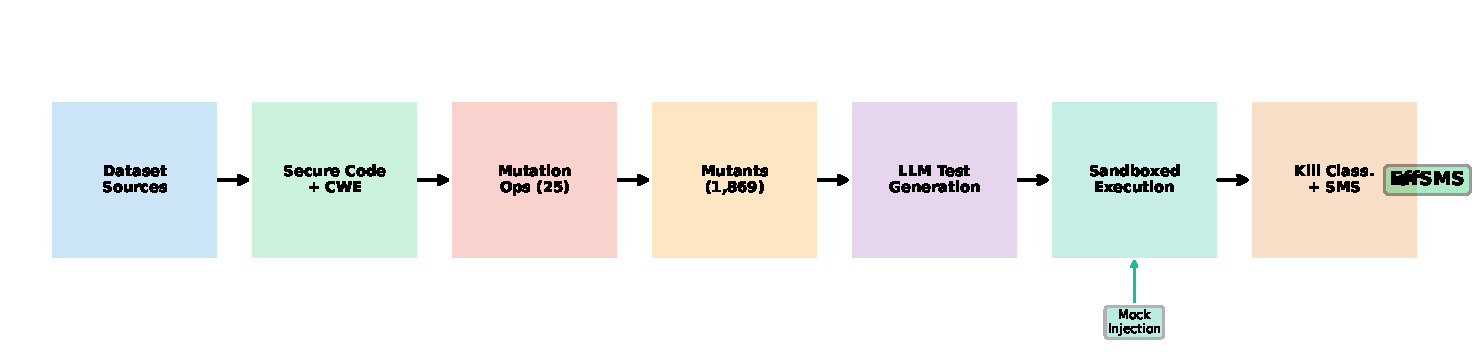
\includegraphics[width=\columnwidth]{figures/framework_overview.pdf}
  \caption{Overview of the SecMutBench evaluation framework. Secure programs are mutated using 25 security-specific operators. LLM-generated tests are executed in sandboxed subprocesses with mock injection, and kills are classified to compute the Effective Security Mutation Score (EffSMS).}
  \label{fig:framework}
\end{figure}

\subsection{Dataset Construction}

SecMutBench consolidates samples from multiple sources to ensure diversity in vulnerability patterns, coding styles, and complexity levels. Table~\ref{tab:dataset} summarizes the dataset composition.

\begin{table}[t]
\caption{Dataset composition by source.}
\label{tab:dataset}
\small
\begin{tabular}{lrl}
\toprule
\textbf{Source} & \textbf{Samples} & \textbf{Description} \\
\midrule
SecMutBench Originals & 75 & Hand-crafted + curated from SecCodePLT, \\
 & & CyberSecEval, SecurityEval \\
CWEval~\cite{yang2024cweval} & 3 & Expert-verified secure/insecure pairs \\
SecurityEval~\cite{siddiq2022securityeval} & 3 & Prompt-based challenges \\
LLM-Generated Variations & 258 & Structurally diverse variants of originals \\
\midrule
\textbf{Total} & \textbf{339} & \textbf{30 CWEs, 1,869 mutants} \\
\bottomrule
\end{tabular}
\end{table}


Each sample contains a secure implementation, an insecure variant with a known vulnerability, CWE classification, reference security tests, and pre-generated mutants. Samples span three difficulty levels: easy (136), medium (101), and hard (102), assigned based on code complexity and vulnerability subtlety.

\textbf{Contamination prevention.} Adapted samples from public sources undergo a four-stage pipeline: temporal CVE filtering (cutoff 2024), CWE-specific structural perturbation, AST-based identifier renaming, and 5-gram Jaccard contamination audit (threshold 0.3). Novel templates and LLM-generated variations (82\% of dataset) are exempt. All perturbations are validated via \texttt{compile()}.

\textbf{LLM-generated variations.} We generated 258 structural variations of original samples using LLMs, each preserving the CWE category and vulnerability mechanism while introducing diverse coding patterns. All variations pass the same validation pipeline (compilation, vulnerability pattern presence, valid mutant generation).

\textbf{CWE selection.} Our 30 CWEs were selected from OWASP Top~10 and CWE Top~25, filtered to Python-relevant vulnerabilities with recent CVEs, retaining only those with implementable mutation operators. The set covers injection, authentication, access control, cryptography, input validation, deserialization, SSRF, CSRF, and 12 additional categories.



\subsection{Security Mutation Operators}

SecMutBench defines 25 mutation operators that transform secure code into vulnerable variants. Unlike traditional mutation operators that create arbitrary syntactic changes~\cite{demillo1978hints}, our operators model specific vulnerability patterns mapped to CWE categories. Table~\ref{tab:operators} presents the operator taxonomy.

Our operators extend the framework of Loise et al.~\cite{loise2017security} (15 Java operators) to Python, adapting three of their operators (PSQLI, RHTTPO, XXE) and introducing 22 new ones covering command injection, deserialization, SSRF, IDOR, CSRF, and 17 additional CWE categories.

\begin{table}[t]
\caption{Security mutation operators (top 15 by mutant count).}
\label{tab:operators}
\small
\begin{tabular}{llr}
\toprule
\textbf{Operator} & \textbf{Target CWEs} & \textbf{n} \\
\midrule
RVALID & CWE-20, 79, 89 & 151 \\
WEAKCRYPTO & CWE-327, 328 & 128 \\
INPUTVAL & CWE-20 & 119 \\
DESERIAL & CWE-502, 94 & 106 \\
RMAUTH & CWE-287, 306 & 105 \\
EVALINJECT & CWE-94, 95 & 98 \\
SSRF & CWE-918 & 97 \\
RENCRYPT & CWE-319, 326 & 90 \\
PATHCONCAT & CWE-22, 73 & 87 \\
MISSINGAUTH & CWE-862, 863 & 83 \\
CSRF\_REMOVE & CWE-352 & 82 \\
HARDCODE & CWE-798 & 81 \\
PSQLI & CWE-89 & 80 \\
OPENREDIRECT & CWE-601 & 63 \\
LOGINJECT & CWE-117 & 62 \\
\bottomrule
\end{tabular}
\vspace{2pt}
{\footnotesize \textit{n} = total mutants produced by operator. Additional operators (NOCERTVALID, WEAKPERM, XXE, LDAPINJECT, WEAKKEY, WEAKRANDOM, FILEUPLOAD, INFOEXPOSE, REGEXDOS, IDOR) produce 20--60 mutants each.}
\end{table}

Each operator implements \texttt{applies\_to(code)} and \texttt{mutate(code)} using pattern-based source transformations rather than AST node replacement, enabling security-specific mutations that tools like MutPy~\cite{derezinska2014experimental} cannot express.

%% Mutation Operator Example (PSQLI, CWE-89)
\begin{figure}[t]
\begin{minipage}[t]{0.48\columnwidth}
\centering\textbf{Secure (original)}
\begin{lstlisting}[numbers=none,frame=single]
def get_user(user_id):
  query = "SELECT * FROM users"
         " WHERE id = %s"
  return db.execute(
      query, (user_id,))
\end{lstlisting}
\end{minipage}%
\hfill
\begin{minipage}[t]{0.48\columnwidth}
\centering\textbf{Mutant (PSQLI)}
\begin{lstlisting}[numbers=none,frame=single]
def get_user(user_id):
  query = f"SELECT * FROM "
   f"users WHERE id={user_id}"
  return db.execute(query)

\end{lstlisting}
\end{minipage}

\smallskip
\small
\noindent\textbf{Kill classifications for this mutant:}
\begin{itemize}\setlength{\itemsep}{0pt}\setlength{\parskip}{0pt}
  \item \textbf{Semantic:} \texttt{assert db.last\_params is not None, "Query should use parameterized execution"}
  \item \textbf{Functional:} \texttt{pytest.raises(ValueError)} --- expected exception no longer raised
  \item \textbf{Incidental:} \texttt{assert len(result) == 5} --- output count changes
  \item \textbf{Crash:} \texttt{TypeError: not all arguments converted during string formatting}
\end{itemize}
\caption{The PSQLI operator transforms a parameterized SQL query (secure, left) into string concatenation (vulnerable, CWE-89, right). Below: illustrative kill classifications showing how the same mutant can be killed via different mechanisms.}
\label{fig:mutation_example}
\end{figure}

Mutants are pre-generated during dataset construction and stored in each sample's JSON record. This ensures deterministic evaluation---the same mutants are used across all evaluation runs---and eliminates variation from operator application order.


\textbf{Mutant validity.} Security operators are structurally less susceptible to equivalent mutants than traditional operators because they transform behavioral security properties~\cite{jia2011analysis,papadakis2019mutation}. All 1,869 mutants (100\%) pass \texttt{compile()} validation and basic execution. The dataset averages 5.51 mutants per program (range 4--9), with each operator targeting a specific vulnerability pattern. Per-operator executability rates are available in the replication package~(\url{https://github.com/Mars-2030/secmutbench}).


\subsection{Kill Classification and SMS Metric}

The central insight of SecMutBench is that not all mutant kills are equal. When a test kills a mutant (passes on secure code, fails on mutant), the kill type reveals whether the test demonstrates genuine security awareness.

Formally, let $P$ denote a secure program and $M = \{m_1, m_2, \ldots, m_k\}$ the set of mutants generated by applying security mutation operators $O = \{o_1, \ldots, o_{25}\}$. For a test suite $T$ generated by an LLM, we define the kill predicate:
\begin{equation}
    \text{kill}(t, m) = \begin{cases} 1 & \text{if } t \text{ passes on } P \text{ and fails on } m \\ 0 & \text{otherwise} \end{cases}
\end{equation}

\noindent For each killed mutant, we classify the failure into one of five categories:

\begin{itemize}\setlength{\itemsep}{2pt}
    \item \textbf{Semantic}: Assertion error with operator-specific security keywords (e.g., ``parameterized'' for PSQLI). The test explicitly checks for the vulnerability.
    \item \textbf{Functional}: Behavioral-contract assertion (expected exception, return type) catches a control-flow change without security framing.
    \item \textbf{Incidental}: Data-value assertion (\texttt{assert len(result)==64}) catches a value change as a side-effect of the mutation.
    \item \textbf{Crash}: Runtime error (TypeError, NameError, ImportError) before any assertion is evaluated.
    \item \textbf{Other}: Residual non-assertion, non-crash exceptions. Excluded from primary metrics.
\end{itemize}

\noindent The five categories are mutually exclusive, assigned in priority order: crash $\rightarrow$ semantic $\rightarrow$ functional $\rightarrow$ incidental $\rightarrow$ other.

\noindent Let $K_s$, $K_f$, $K_i$, $K_c$, and $K_o$ denote the sets of semantic, functional, incidental, crash, and other kills respectively, where $K_s \cup K_i \cup K_f \cup K_c \cup K_o \subseteq M$ and the sets are mutually disjoint. We define the \textbf{Security Mutation Score} as:
\begin{equation}
    \text{SMS} = \frac{|K_s|}{|M|}
\end{equation}

\noindent In contrast, the traditional Mutation Score (MS) counts all kills:
\begin{equation}
    \text{MS} = \frac{|K_s| + |K_i| + |K_f| + |K_c| + |K_o|}{|M|}
\end{equation}

\noindent The \textbf{inflation ratio} $\rho$ captures the overstatement:
\begin{equation}
    \rho = \frac{\text{MS}}{\text{SMS}}
\end{equation}

\noindent When $\rho \gg 1$, the gap is attributable to crash, functional, incidental, and other kills that do not represent genuine security detection.

Because SMS is computed only over samples where the generated test suite passes on secure code, it does not penalize models for producing invalid tests. To capture practical end-to-end effectiveness, we define the \textbf{Effective Security Mutation Score}:
\begin{equation}
    \text{EffSMS} = \text{SMS} \times \text{SPR}
\end{equation}
\noindent where SPR (Secure-Pass Rate) is the proportion of samples for which the generated test suite passes on the secure code. EffSMS is the primary comparability metric: it reflects how much security-aware detection a model delivers \emph{across the entire benchmark}, accounting for both test validity and security awareness. We additionally report SMS and SPR separately for diagnostic decomposition.

\textbf{Vulnerability Detection (VD).} As a ground-truth sanity check, we compute a binary Vulnerability Detection metric that verifies whether generated tests can distinguish secure from insecure code:
\begin{equation}
    \text{VD}(p) = \begin{cases} 1 & \text{if } T_p \text{ passes on } P_p^{\text{sec}} \text{ and fails on } P_p^{\text{insec}} \\ 0 & \text{otherwise} \end{cases}
\end{equation}

\noindent and report the aggregate $\text{VD} = |\{p : \text{VD}(p) = 1\}| / |P|$. Note that VD is \emph{not} a mutation-based metric---it tests against the original insecure code, not mutants. Mutant-based vulnerability detection is captured by MS and SMS.

\textbf{Operator-aware classification.} A key refinement in SecMutBench is that kill classification uses operator-specific keyword lists rather than a flat global list. For example, ``path'' triggers semantic classification only for \textsc{PATHCONCAT} mutants, not for \textsc{PSQLI} mutants. Each of the 25 operators has a tailored set of security-relevant terms (e.g., \textsc{WEAKCRYPTO}: \{md5, sha1, weak, bcrypt, salt\}; \textsc{DESERIAL}: \{pickle, yaml, safe\_load, SafeLoader\}). This prevents false inflation of SMS scores from coincidental keyword matches. Complete operator specifications, keyword lists, and LLM-as-Judge evaluation prompts are available in the replication package at \url{https://github.com/Mars-2030/secmutbench}.


\subsection{Evaluation Pipeline}

The pipeline executes LLM-generated tests in isolated subprocesses with 11 CWE-specific mock environments injected via \texttt{sys.modules} and builtins patching. Mocks serve dual purposes: \emph{safety} (blocking real system calls via a \texttt{SafeOS} wrapper) and \emph{observability} (tracking security-relevant operations, e.g., \texttt{db.last\_params}, \texttt{subprocess.last\_shell}). For each sample: (1)~tests run against secure code (should pass), (2)~tests run against each mutant (should fail), (3)~kills are classified via operator-aware heuristics, and (4)~SMS/EffSMS are computed.



%% ====================================================================
%% IV. EXPERIMENTAL SETUP
%% ====================================================================
\section{Experimental Setup}\label{sec:setup}

\subsection{Research Questions}

\begin{description}
    \item[RQ1:] \textit{How effectively do LLMs generate security-aware tests?} We compare overall mutation scores (MS) against Security Mutation Scores (SMS) to quantify the inflation introduced by functional, incidental, and crash kills.

    \item[RQ2:] \textit{What types of kills do LLM-generated tests produce?} We analyze the kill classification breakdown to understand why traditional metrics overstate LLM security testing capability.

    \item[RQ3:] \textit{How does security test effectiveness vary across vulnerability types?} We examine per-CWE and per-operator effectiveness to identify systematic blind spots, including comparison with static analysis baselines.


    \item[RQ4:] \textit{How sensitive is SMS to prompt design and how do LLMs compare to human-written tests?} We ablate prompt detail levels (no hint, CWE ID only, full context) and compare LLM-generated tests against expert-written reference tests to establish upper bounds. 

\end{description}


\subsection{Subject Models}

We evaluate eight LLMs spanning open-weight and proprietary models, plus two static analysis baselines. Table~\ref{tab:models} summarizes the models. All LLMs are evaluated in a zero-shot setting with temperature 0 (greedy decoding) and maximum 2048 output tokens.

\begin{table}[t]
\caption{Subject models and baselines.}
\label{tab:models}
\small

\begin{tabular}{lllll}
\toprule
\textbf{Model} & \textbf{Version / ID} & \textbf{Size} & \textbf{Provider} & \textbf{Access} \\
\midrule
GPT-oss-120B & \texttt{gpt-oss-120b} & 120B & OpenAI & API \\
GPT-5.2 & \texttt{gpt-5.2-2025-12-11} & -- & OpenAI & API \\
GPT-5-mini & \texttt{gpt-5-mini-2025-08-07} & -- & OpenAI & API \\
Qwen3-Coder & \texttt{qwen3-coder:30b} & 30B & Alibaba & Ollama \\
Qwen2.5-Coder & \texttt{qwen2.5-coder:14b-instruct} & 14B & Alibaba & Ollama \\
Kimi-K2.5 & \texttt{kimi-k2.5:cloud} & -- & Moonshot & Ollama \\
GLM-5 & \texttt{glm-5:cloud} & -- & Zhipu AI & Ollama \\
DeepSeek-Coder-V2 & \texttt{deepseek-coder-v2:latest} & 236B MoE & DeepSeek & Ollama \\
\midrule
Bandit & 1.9.2 & -- & Static & CLI \\
Semgrep & -- & -- & Static & CLI \\
\bottomrule
\end{tabular}

\end{table}

Open-weight models are served locally via Ollama providing an OpenAI-compatible API. Proprietary models are accessed via their respective cloud APIs. All kill classifications are validated using an LLM-as-Judge (GPT-5.4) to reclassify heuristic labels.


\subsection{Prompting Strategy}

Each model receives a zero-shot prompt containing the secure code, CWE identifier/name, and mock environment documentation with detection patterns (e.g., \texttt{db.last\_params is not None} for SQL injection). We evaluate three prompt variants: (a)~\emph{full context} (default, with mock docs and assertion guidance), (b)~\emph{CWE-ID only} (``Write tests to detect CWE-89''), and (c)~\emph{no hint} (``Write tests for this function''). The complete prompt template is available in the replication package.



\subsection{Baselines}

We include three baselines: (1) \textbf{Bandit}~\cite{bandit2024}, a widely-used Python static analysis tool, run on insecure code to measure detection rate per CWE; (2) \textbf{Semgrep}~\cite{semgrep2024} with the \texttt{p/security-audit} ruleset, providing a second static analysis comparison with broader rule coverage; and (3) \textbf{Reference tests}, the expert-written security tests included in each SecMutBench sample, establishing an upper-bound baseline for what hand-crafted security tests achieve on our mutants.


Bandit detects 77 of 339 samples (22.7\% overall detection rate). On the 11 static-analyzable CWEs (147 samples), Bandit achieves 71.4\% detection; on the remaining 19 dynamic-only CWEs (192 samples), Bandit achieves 0\% detection. Semgrep with \texttt{p/python} rules detects 37 samples (10.9\%). Reference tests achieve MS of 57.7\% and SMS of 47.6\% (889 semantic kills out of 1,869 mutants), establishing the expert upper bound.



\subsection{Execution Environment}

All experiments use Python~3.11.5 on macOS with 5-second test timeouts. Each model evaluates all 339 samples across three prompt variants in a single run with temperature~0 (greedy decoding), producing deterministic outputs (seed~42). Secure-pass rates range from 7.1\% (DeepSeek) to 46.6\% (Qwen3); tests failing on secure code are excluded from mutation evaluation.


%% ====================================================================
%% V. RESULTS
%% ====================================================================
\section{Results}\label{sec:results}

\subsection{RQ1: Overall Effectiveness}

Table~\ref{tab:rq1} presents the overall results. Effective SMS (EffSMS = SMS $\times$ SPR) is the primary comparability metric, capturing end-to-end security testing effectiveness across the entire benchmark. SMS and SPR are reported separately for diagnostic decomposition.

\begin{table}[t]
\caption{Overall results (OpenAI-judged, full-context prompt). EffSMS = SMS $\times$ SPR is the primary metric.}
\label{tab:rq1}
\small

\begin{tabular}{lrrrrr}
\toprule
\textbf{Model} & \textbf{MS} & \textbf{SPR} & \textbf{EffSMS} & \textbf{SMS} & \textbf{MS/SMS} \\
\midrule
Qwen3-Coder 30B & 75.2 & 46.6 & \textbf{19.7} & 42.3 & 1.78 \\
Kimi-K2.5 & 84.2 & 42.8 & 19.6 & 45.7 & 1.84 \\
GPT-oss-120B & 90.0 & 36.0 & 15.6 & 43.2 & 2.08 \\
GPT-5-mini & 84.2 & 29.2 & 11.6 & 39.8 & 2.12 \\
Qwen2.5-Coder 14B & 83.6 & 16.8 & 9.8 & 58.6 & 1.43 \\
GLM-5 & 40.0 & 33.0 & 9.0 & 27.4 & 1.46 \\
GPT-5.2 & 88.7 & 13.3 & 5.1 & 38.3 & 2.32 \\
DeepSeek-Coder-V2 & 51.7 & 7.1 & 0.8 & 10.9 & 4.74 \\
\midrule
Reference Tests & 57.7 & 100.0 & \textbf{47.6} & 47.6 & 1.21 \\
Bandit & 22.7 & -- & -- & -- & -- \\
\bottomrule
\end{tabular}

\vspace{2pt}
{\footnotesize Models sorted by EffSMS (descending). \textbf{MS}~=~Mutation Score (all kills). \textbf{SPR}~=~Secure-Pass Rate (\% of tests passing on secure code). \textbf{EffSMS}~=~Effective SMS (SMS $\times$ SPR). \textbf{SMS}~=~Security Mutation Score (semantic kills only, among valid tests). All values are percentages.}
\end{table}


The headline result is the gap between expert-written and LLM-generated tests. Reference tests achieve 47.6\% EffSMS; the best LLM (Qwen3-Coder~30B) achieves 19.7\%---a 2.4$\times$ gap that raw MS completely obscures (reference MS of 57.7\% is \emph{lower} than six of eight LLMs). The ranking by EffSMS differs strikingly from the ranking by MS: GPT-5.2, which ranks second on MS (88.7\%), drops to seventh on EffSMS (5.1\%) because only 13.3\% of its tests are valid. Conversely, Qwen3-Coder ranks sixth on MS but first on EffSMS, because its 46.6\% SPR compensates for moderate SMS.

Among valid test suites, the inflation ratio (MS/SMS) ranges from 1.43 (Qwen2.5-Coder) to 4.74 (DeepSeek-Coder-V2), with a mean of 2.2$\times$. Qwen2.5-Coder achieves the highest SMS (58.6\%)---exceeding reference tests (47.6\%)---but its 16.8\% SPR yields only 9.8\% EffSMS, demonstrating that raw SMS without test validity is misleading.


\smallskip\noindent\fbox{\parbox{0.95\columnwidth}{\textbf{Finding 1a (generation quality):} Only 7--47\% of LLM-generated test suites pass on secure code. Accounting for this, the best EffSMS is 19.7\% (Qwen3-Coder), compared to 47.6\% for expert-written reference tests---a 2.4$\times$ gap that raw mutation scores completely obscure.}}\smallskip

\smallskip\noindent\fbox{\parbox{0.95\columnwidth}{\textbf{Finding 1b (when tests are valid):} Among valid test suites, traditional MS overstates security testing capability by 2.2$\times$ on average (range 1.4--4.7$\times$). The best model when tests are valid is Qwen2.5-Coder (58.6\% SMS), but its 16.8\% SPR makes its practical EffSMS only 9.8\%.}}\smallskip


\subsection{RQ2: Kill Classification Analysis}

Table~\ref{tab:kills} presents the kill classification breakdown for each model's full-context prompt variant. Kill counts reflect only the mutants from samples where the model's tests passed on secure code.

\begin{figure}[t]
  \centering
  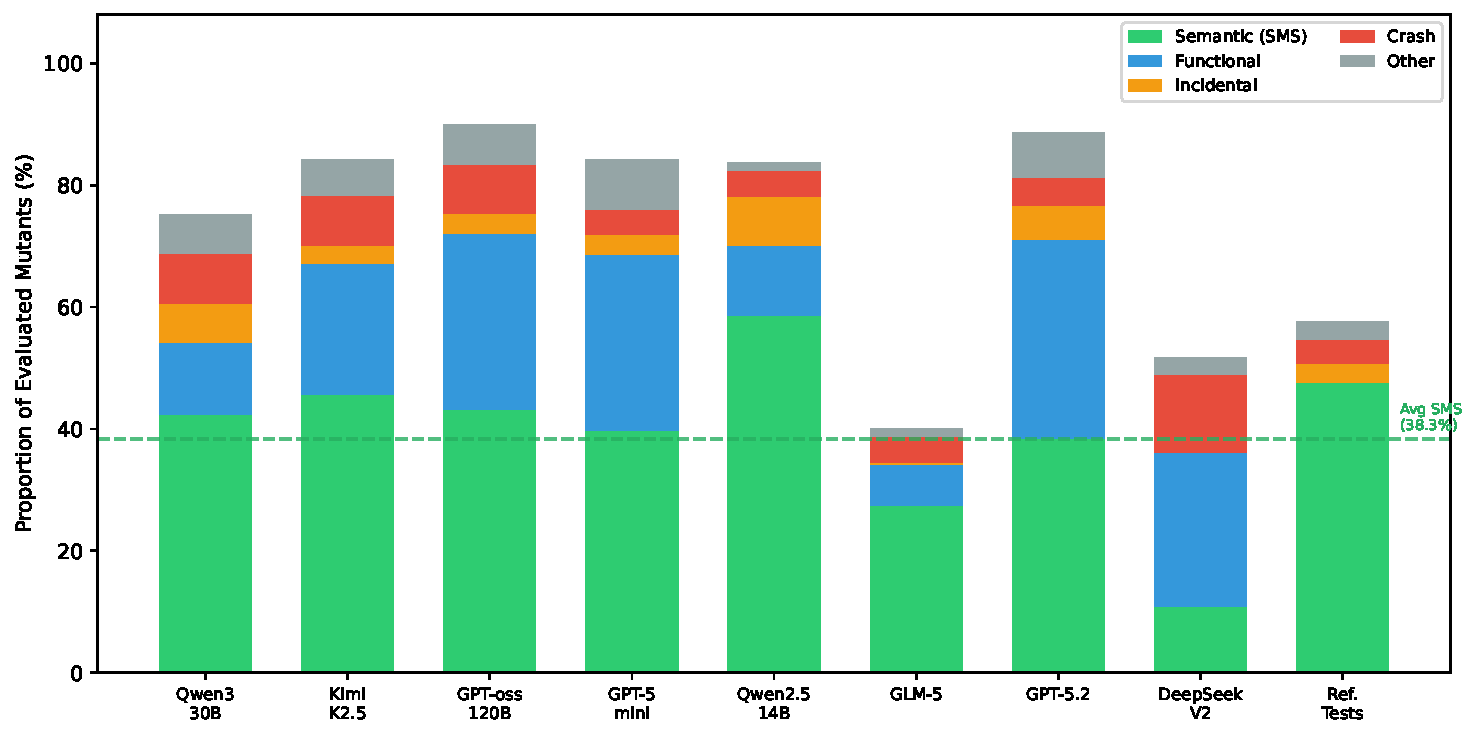
\includegraphics[width=\columnwidth]{figures/kill_breakdown.pdf}
  \caption{Kill classification breakdown across evaluated models. The green segment (semantic kills) represents SMS; the gap between total bar height (MS) and the green segment illustrates the inflation ratio. Dashed line shows average SMS across LLMs.}
  \label{fig:kills}
\end{figure}


\begin{table}[t]
\caption{Kill classification breakdown (full-context prompt, counts).}
\label{tab:kills}
\small
\begin{tabular}{lrrrrrr}
\toprule
\textbf{Model} & \textbf{Mut.} & \textbf{Sem.} & \textbf{Func.} & \textbf{Incid.} & \textbf{Crash} & \textbf{Other} \\
\midrule
GPT-oss-120B & 672 & 290 & 194 & 22 & 54 & 45 \\
GPT-5.2 & 266 & 102 & 87 & 15 & 12 & 20 \\
GPT-5-mini & 538 & 214 & 155 & 18 & 22 & 44 \\
Kimi-K2.5 & 795 & 363 & 171 & 23 & 66 & 46 \\
Qwen2.5 14B & 324 & 190 & 37 & 26 & 14 & 4 \\
Qwen3 30B & 839 & 355 & 100 & 53 & 69 & 54 \\
DeepSeek-V2 & 147 & 16 & 37 & 0 & 19 & 4 \\
GLM-5 & 610 & 167 & 41 & 2 & 26 & 8 \\
\midrule
Reference & 1869 & 889 & 0 & 60 & 73 & 56 \\
\bottomrule
\end{tabular}
\vspace{2pt}
{\footnotesize \textbf{Mut.}~=~mutants evaluated (from valid-test samples). \textbf{Sem.}~=~semantic kills. \textbf{Func.}~=~functional kills. \textbf{Incid.}~=~incidental. Reference tests evaluate all 1,869 mutants (100\% SPR).}
\end{table}



Functional kills---not crashes---dominate non-semantic kills for LLM-generated tests (15--36\% of all kills), while reference tests produce zero functional kills. For GPT-oss-120B, functional kills (194) exceed crash kills (54). Qwen2.5-Coder has the lowest non-semantic proportion (29.9\%).




\textbf{Example.} A Kimi-K2.5 test asserts \texttt{not hashlib.weak\_algorithm\_used} after calling a hashing function. The WEAKCRYPTO mutant substitutes \texttt{sha256} with \texttt{md5}, causing the mock to set \texttt{weak\_algorithm\_used = True}---a semantic kill via mock observability. By contrast, a functional kill on the same mutant would catch it via \texttt{assert len(result)==64} (output length change), and a crash kill via \texttt{NameError} (removed computation line).



\textbf{Classification audit.} Rather than relying solely on heuristic keyword matching, we validate all kill classifications using an LLM-as-Judge (GPT-5.4). The judge receives each kill's error message, operator, CWE, and test code, and independently classifies it into semantic, functional, incidental, crash, or other. All results reported in this paper use the judge-validated classifications. We additionally performed a human validation study on a stratified sample of 120 kills to assess heuristic--annotator agreement, yielding Cohen's $\kappa = 0.502$ (moderate agreement).

Table~\ref{tab:ira} shows per-operator agreement, revealing a
systematic pattern rather than random noise: \emph{syntactic}
operators (PSQLI, WEAKPERM, LOGINJECT, DESERIAL) achieve 89--100\%
agreement, while \emph{behavioral} operators (IDOR, OPENREDIRECT,
MISSINGAUTH, SSRF) achieve 0--17\% agreement. This split directly
reflects whether the kill's security intent is visible in the error
message (syntactic operators produce assertion failures with
security-relevant terms) or only in the test logic (behavioral
operators produce \texttt{DID NOT RAISE} failures with no security-specific
content). The disagreement is therefore \emph{structurally
predictable} from operator type, not from annotator subjectivity.

\begin{table}[t]
\caption{Per-operator annotator--heuristic agreement on kill
classification. Syntactic operators (top) show near-perfect
agreement; behavioral operators (bottom) show systematic divergence
driven by the \texttt{DID NOT RAISE} classification gap.}
\label{tab:ira}
\small
\setlength{\tabcolsep}{4pt}
\begin{tabular}{llrrr}
\toprule
\textbf{Operator} & \textbf{Type} &
\textbf{n} &
\textbf{Annot.\ sem.} &
\textbf{Agreement} \\
\midrule
PSQLI        & Syntactic &  7 & 100\% & 100\% \\
WEAKPERM     & Syntactic &  9 & 100\% & 100\% \\
LOGINJECT    & Syntactic &  3 & 100\% & 100\% \\
DESERIAL     & Syntactic & 18 &  17\% &  89\% \\
WEAKRANDOM   & Syntactic &  4 &  75\% &  75\% \\
\midrule
RVALID       & Behavioral & 11 &  27\% &  64\% \\
PATHCONCAT   & Behavioral &  3 &  33\% &  67\% \\
SSRF         & Behavioral & 13 &  46\% &  54\% \\
EVALINJECT   & Behavioral &  8 &  13\% &  50\% \\
XXE          & Behavioral &  4 &  50\% &  50\% \\
INPUTVAL     & Behavioral & 15 &  53\% &  47\% \\
MISSINGAUTH  & Behavioral &  6 & 100\% &  17\% \\
OPENREDIRECT & Behavioral &  4 & 100\% &   0\% \\
IDOR         & Behavioral &  7 & 100\% &   0\% \\
\bottomrule
\end{tabular}
\vspace{3pt}
{\footnotesize \textbf{Annot.\ sem.}: proportion of kills the
annotator labeled semantic. \textbf{Agreement}: proportion where
annotator and heuristic agree. For behavioral operators where
annotator labels semantic but heuristic labels functional (e.g.,
SSRF, IDOR, OPENREDIRECT), the heuristic is conservative: it misses
semantic kills whose security intent is expressed in the test logic
rather than the error message. The LLM-as-Judge reclassification
corrects this conservative bias for the reported results.}
\end{table}



\smallskip\noindent\fbox{\parbox{0.95\columnwidth}{\textbf{Finding 2:} Functional kills---not crash kills---are the dominant non-semantic category for LLM-generated tests, accounting for 15--36\% of all kills. Reference tests produce zero functional kills. This reveals that LLMs often detect mutations through behavioral side-effects rather than security-targeted assertions.}}\smallskip


\subsection{RQ3: Vulnerability-Specific Analysis}

Table~\ref{tab:rq3} presents per-CWE effectiveness aggregated across models, alongside Bandit detection rates. CWEs are grouped by whether they are amenable to static analysis (pattern-based) or require dynamic behavioral testing (logic-flaw).

\begin{table}[t]
\caption{Per-CWE effectiveness (selected CWEs, aggregated across models).}
\label{tab:rq3}
\small
\begin{tabular}{llrrr}
\toprule
\textbf{CWE} & \textbf{Category} & \textbf{n} & \textbf{Mut.} & \textbf{Bandit} \\
\midrule
CWE-89 & SQL Injection & 16 & 80 & 71.4\% \\
CWE-22 & Path Traversal & 15 & 87 & 71.4\% \\
CWE-94 & Code Injection & 15 & 102 & 71.4\% \\
CWE-327 & Weak Crypto & 12 & 71 & 71.4\% \\
CWE-798 & Hardcoded Creds & 13 & 81 & 71.4\% \\
\midrule
CWE-306 & Missing Auth & 16 & 97 & 0\% \\
CWE-352 & CSRF & 14 & 82 & 0\% \\
CWE-862 & Missing Authz & 10 & 62 & 0\% \\
CWE-639 & IDOR & 5 & 20 & 0\% \\
CWE-918 & SSRF & 15 & 97 & 0\% \\
\bottomrule
\end{tabular}
\vspace{2pt}
{\footnotesize Top group: static-analyzable CWEs (Bandit achieves 71.4\% detection). Bottom group: logic-flaw CWEs (Bandit achieves 0\%). \textbf{n}~=~samples, \textbf{Mut.}~=~total mutants. Full 30-CWE breakdown available in the replication package~(\url{https://github.com/Mars-2030/secmutbench}).}
\end{table}

Bandit achieves 71.4\% detection on 11 pattern-based CWEs but 0\% on 19 logic-flaw CWEs. CWE-89 achieves 100\% SMS across all models; CWE-611 (XXE) and CWE-95 are universal blind spots at 0\% SMS (Figure~\ref{fig:cwe_heatmap}).


\begin{figure}[t]
  \centering
  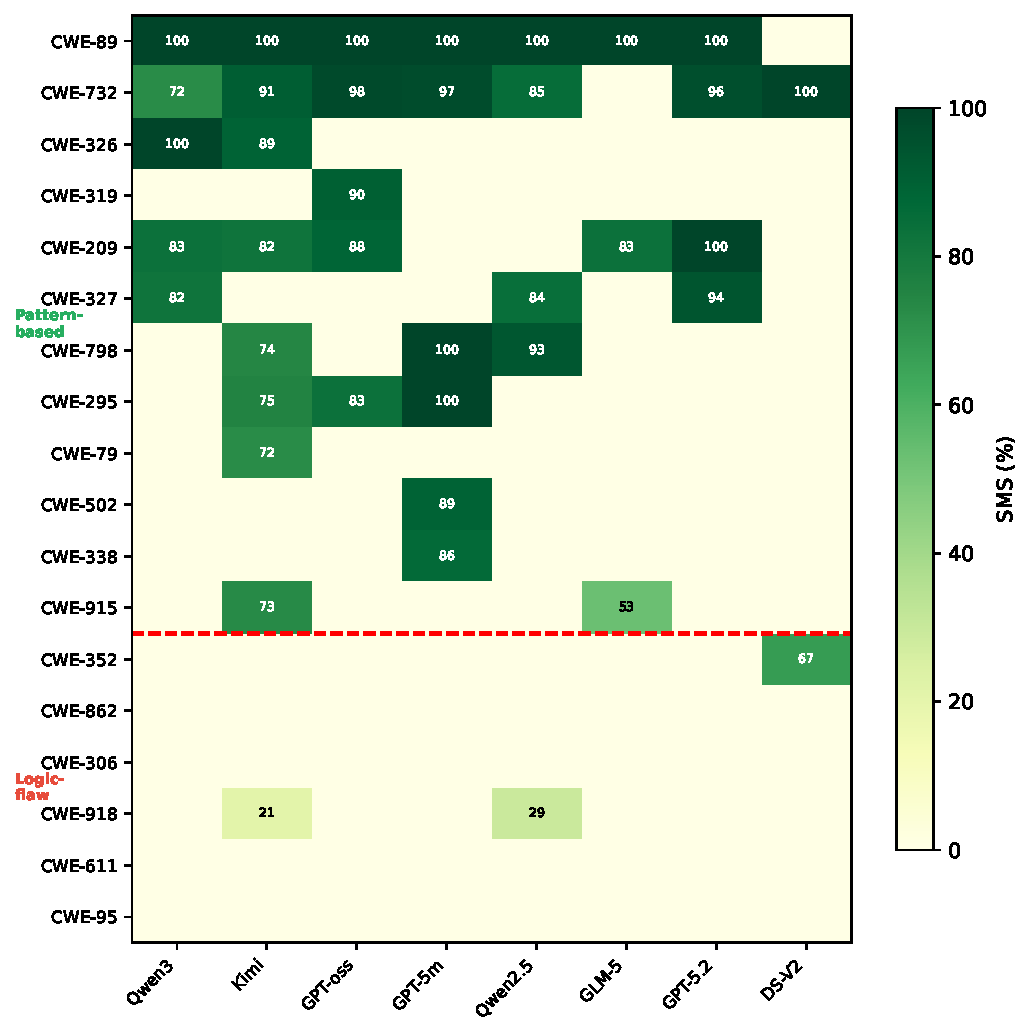
\includegraphics[width=\columnwidth]{figures/cwe_heatmap.pdf}
  \caption{Per-CWE Security Mutation Score across models. Pattern-based CWEs (above dashed line) vs.\ logic-flaw CWEs (below) reveal distinct detection profiles. CWE-89 achieves 100\% SMS across all models; CWE-611 and CWE-95 are universal blind spots at 0\%.}
  \label{fig:cwe_heatmap}
\end{figure}

\smallskip\noindent\fbox{\parbox{0.95\columnwidth}{\textbf{Finding 3:} Static analysis (Bandit) achieves 71.4\% detection on 11 pattern-based CWEs but 0\% on 19 logic-flaw CWEs. LLM-generated tests provide complementary coverage on logic-flaw vulnerabilities (authentication, authorization, CSRF, SSRF) where static analysis is structurally blind.}}\smallskip


\subsection{RQ4: Prompt Sensitivity}

Table~\ref{tab:ablation} compares SMS across three prompt variants. No-hint prompts consistently degrade SMS (average delta of 24.8~pp vs.\ best variant), with GPT-oss dropping to 0\%. Explicit vulnerability guidance is essential for security-aware test generation.

\begin{table}[t]
\caption{Prompt ablation: SMS (\%) by prompt variant.}
\label{tab:ablation}
\small
\begin{tabular}{lrrr}
\toprule
\textbf{Model} & \textbf{No hint} & \textbf{CWE ID} & \textbf{Full context} \\
\midrule
GPT-oss-120B & 0.0 & 52.3 & 43.2 \\
GPT-5.2 & 31.2 & 54.5 & 38.3 \\
GPT-5-mini & 20.7 & 38.1 & 39.8 \\
Kimi-K2.5 & 30.1 & 57.5 & 45.7 \\
Qwen2.5-Coder 14B & 12.9 & 14.9 & 58.6 \\
Qwen3-Coder 30B & 35.5 & 42.5 & 42.3 \\
DeepSeek-Coder-V2 & 7.1 & 7.5 & 10.9 \\
GLM-5 & 25.6 & 34.3 & 27.4 \\
\bottomrule
\end{tabular}
\end{table}

\smallskip\noindent\fbox{\parbox{0.95\columnwidth}{\textbf{Finding 4:} No-hint prompts severely degrade SMS (0--35.5\%). Expert reference tests achieve 47.6\% EffSMS; the best LLM reaches only 19.7\% EffSMS.}}\smallskip


%% ====================================================================
%% VI. DISCUSSION
%% ====================================================================
\section{Discussion}\label{sec:discussion}

The 2.4$\times$ EffSMS gap between expert-written tests (47.6\%) and the best LLM (19.7\%) compounds from two sources: most generated tests fail on secure code (SPR 7--47\%), and among valid tests, functional kills and crashes inflate MS by 2.2$\times$ over SMS. A model reporting 90\% MS may deliver only 5\% EffSMS (GPT-5.2: 88.7\% $\rightarrow$ 5.1\%). This extends Mouelhi et al.'s~\cite{mouelhi2007mutation} finding that functional tests fail to achieve high security mutation scores: LLMs proficient at generating functional tests may nevertheless lack genuine security reasoning.

\textbf{Static analysis complementarity.} Bandit achieves 71.4\% detection on 11 syntactic CWEs but 0\% on 19 logic-flaw CWEs. Running Bandit on mutants rather than insecure originals would not change this: syntactic operators (PSQLI, WEAKCRYPTO) introduce the same patterns Bandit detects in originals, while behavioral operators (MISSINGAUTH, IDOR, CSRF\_REMOVE) produce \emph{missing logic} undetectable by any static rule. LLMs provide unique value on logic-flaw CWEs (e.g., CWE-306: Kimi 75\% SMS, CWE-732: GPT-5-mini 97\%).

\textbf{SMS robustness.} SMS could theoretically be gamed by inserting security keywords without genuine understanding. Three structural mitigations prevent this: (1)~operator-aware keywords prevent cross-CWE gaming; (2)~the kill predicate requires tests to pass on secure code \emph{and} fail on the mutant; (3)~mock state tracking supports future observability-based classification. We recommend that evaluations decompose kills by type, use pre-generated mutants for reproducibility, and review LLM-generated tests for security-specific assertions rather than trusting pass/fail behavior alone.


%% ====================================================================
%% VIII. THREATS TO VALIDITY
%% ====================================================================
\section{Threats to Validity}\label{sec:threats}

\textbf{Internal validity.} Kill classification may misclassify kills where security terms appear coincidentally or where genuine assertions use non-standard terminology. We mitigate this with operator-aware keywords, an LLM-as-Judge (GPT-5.4) reclassification, and a human validation study ($\kappa = 0.502$; Table~\ref{tab:ira}). Disagreement is structurally predictable by operator type (syntactic: 89--100\% agreement; behavioral: 0--17\%), not random.
%
\textbf{External validity.} SecMutBench covers 30 CWEs in Python only; temperature-0 single-run evaluation produces deterministic results but may not generalize to stochastic settings. Our contamination pipeline mitigates training-data overlap but cannot guarantee zero contamination for all models.
%
\textbf{Construct validity.} The mock environment introduces an ecological validity gap---most clearly for CWE-611 (XXE), which achieves 0\% SMS across all models due to API mismatch between MockXMLParser and real parsers. Mock-dependent SMS values should be treated as conservative lower bounds. All 1,869 mutants pass compilation (100\% executable mutant ratio); equivalent mutants are structurally unlikely for security operators but may occur for validation-removal operators on unreachable paths.




%% ====================================================================
%% IX. CONCLUSION
%% ====================================================================
\section{Conclusion}\label{sec:conclusion}

We presented SecMutBench, a mutation-based benchmark with 25 operators, 339 programs, 30 CWEs, and 1,869 mutants for evaluating LLM-generated security tests. The best LLM achieves only 19.7\% EffSMS compared to 47.6\% for expert-written tests---a 2.4$\times$ gap compounding from low test validity (SPR 7--47\%) and MS/SMS inflation (2.2$\times$). Static analysis and mutation testing provide complementary coverage: Bandit excels on 11 syntactic CWEs (71.4\%) while LLMs cover 19 logic-flaw CWEs where Bandit achieves 0\%. Future work includes multi-language support, observability-based kill classification via mock state tracking, and iterative refinement with surviving mutants~\cite{dakhel2023mutap,mutgen2025}. The code and replication package are at \url{https://github.com/Mars-2030/secmutbench}; the dataset is at \url{https://huggingface.co/datasets/Mars203020/secmutbench}.



%%
%% The acknowledgments section is defined using the "acks" environment
%% (and NOT an unnumbered section). This ensures the proper
%% identification of the section in the article metadata, and the
%% consistent spelling of the heading.
\begin{acks}
Large language models (Claude Code and ChatGPT) were used as development tools during this work: to assist in writing the benchmark's evaluation pipeline and mutation operator code, to edit and revise drafts of this paper, and to generate the figures. All LLM-assisted outputs were reviewed and validated by the authors.
\end{acks}

%%
%% The next two lines define the bibliography style to be used, and
%% the bibliography file.
\bibliographystyle{ACM-Reference-Format}
\bibliography{ref}


%%
%% If your work has an appendix, this is the place to put it.
\appendix




\end{document}
\endinput
%%
%% End of file `sample-sigconf.tex'.
